\newpage
\section{Protokollmechanismen 1}
  \subsection{Grundlegende Begriffe}
    \subsubsection{Datenkommunikation}
      \begin{itemize}
        \item Datenkommunikation dient dem Austausch von Daten über (größere) Distanzen
          \begin{itemize}
            \item Die Distanzen werden durch Übertragungsmedien überbrückt
            \item Der Datenaustausch erfolgt entsprechend definierter Protokolle
          \end{itemize}
      \end{itemize}
      \subsubsection{(Kommunikations-)Protokoll}
      \begin{itemize}
        \item Protokolle definieren Regeln und Formate für die Kommunikation (Interaktion) zwischen
          zwei oder mehr Computern sowie die beim Senden bzw. Empfangen von Daten bzw. Ereignissen
          jeweils durchzuführenden Aktionen
          \begin{itemize}
            \item Regeln definieren den zeitlichen Ablauf sowie die Aktionen
            \item Formate definieren Syntax und Semantik der ausgetauschten Daten
          \end{itemize}
        \item Protokolle können durch Hardware, Software oder eine Kombination von beidem implementiert
          werden
      \end{itemize}
    \subsubsection{Wet-Zeit-Diagramm}
      \begin{itemize}
        \item Grafische Darstellung räumlich verteilter Abläufe innerhalb eines 
          2-Achsen-Koordinatensystems
          \begin{itemize}
            \item Vertikale Achse: Zeitachse
              \begin{itemize}
                \item Abstrahiert meist vom tatsächlichen Zeitpunkt
              \end{itemize}
            \item Horizontale Achse: Räumliche Distanz
              \begin{itemize}
                \item Abstrahiert von der tatsächlich räumlichen Distanz
              \end{itemize}
          \end{itemize}
        \item Vorwiegend für einfachere Sachverhalte geeignet, dort aber sehr hilfreich
        \item Darstellung von Alternativen
          \begin{itemize}
            \item In einem Weg-Zeit-Diagramm schnell übersichtlich
            \item Typischerweise je Sachverhalt separates Weg-Zeit-Diagramm
          \end{itemize}
          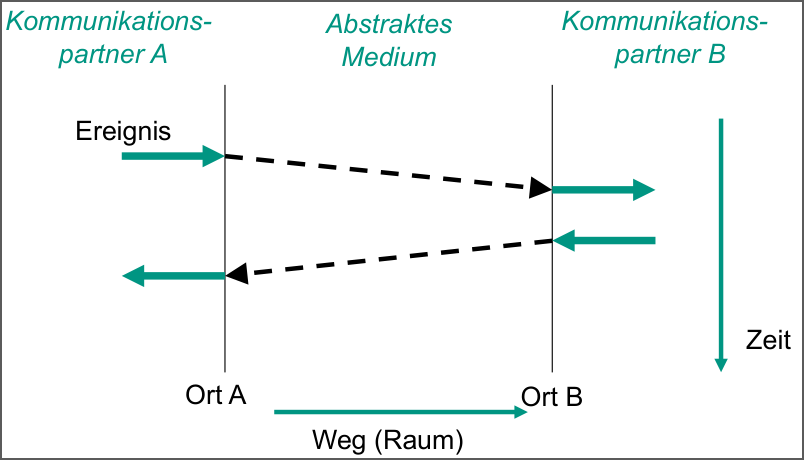
\includegraphics[width=\textwidth]{img/weg_zeit.png}
      \end{itemize}
  \subsection{Zuverlässigkeit (Reliability)}
    Zuverlässige Auslieferung (Reliable Delivery)
    \begin{itemize}
      \item Pakete können Bitfehler aufweisen oder verloren gehen, z.B. durch
        \begin{itemize}
          \item Überlastete Links
          \item Nicht funktionierende Router
        \end{itemize}
      \item Zuverlässigkeit gefordert, dann
        \begin{itemize}
          \item Sendewiederholung durch Sender notwendig
          \item Hierzu: Sender muss über Verlust (bzw. nicht verlust) informiert werden
            \begin{itemize}
              \item Quittungen vom Empfänger (z.B. positive Quittung, Acknowledgement (ACK))
              \item Timeout beim Sender wenn keine Quittung zu Paket empfangen $\ra$ Sendewiederholung
              \item Sequenznummern, um Paket zu identifizieren
            \end{itemize}
        \end{itemize}
    \end{itemize}
    \subsubsection{Fehlerbehaftete Kommunikation}
      Paketfehler - Fehlerarten
      \begin{itemize}
        \item Verlust eines Paketes
        \item Empfang eines Phantom-Paketes
        \item Duplizierung eines Paketes
        \item Reihenfolgenvertausschung
      \end{itemize}
      Bitfehler
      \begin{itemize}
        \item Verfälschung von Bits während der Übertragung
          \begin{itemize}
            \item Z.B. "0" vom Sender gesendet und "1" vom Empfänger empfangen
            \item Fehlerursachen
              \begin{itemize}
                \item Dämpfung des Übertragungssignals, Übersprechen, Verlust der Bit-Synchronisatoin
              \end{itemize}
          \end{itemize}
        \item Einzelbitfehler
          \begin{itemize}
            \item Ein einzelnes Bit ist fehlerhaft
          \end{itemize}
        \item Bündelfehler
          \begin{itemize}
            \item Mehrere direkt aufeinaderfolgende Bits sind fehlerhaft
          \end{itemize}
      \end{itemize}
    \subsubsection{Zuverlässiger (Kommunikations-)Dienst}
      Definition
      \begin{itemize}
        \item Bei einem zuverlässigen (Kommunikations-)Dienst gilt am entsprechenden Dienstzugangspunkt
          des Empfängers folgendes
          \begin{itemize}
            \item Alle empfangenen Daten sind korrekt
            \item Alle vom Sender gesendeten Daten werden vollständig und in der richtigen
              Reihenfolge (d.h. Reihenfolge des Senders) empfangen
            \item Es werden keine Duplikate empfangen
            \item Es werden keine Phantom-Daten empfangen
          \end{itemize}
      \end{itemize}
      \pagebreak
      Sequenznummern
      \begin{itemize}
        \item Problem
          \begin{itemize}
            \item Woher weiß der Empfänger, ob
              \begin{itemize}
                \item Pakete in der richtigen Reihenfolge ankommen?
                \item Duplikate enthalten sind?
                \item Pakete fehlen?
              \end{itemize}
          \end{itemize}
        \item Mechanismus
          \begin{itemize}
            \item Pakete (oder Bytes) werden nummeriert
            \item Entsprechende Kennung (Sequenznummer) wird mit jedem Paket übertragen
          \end{itemize}
        \item Anzahl der Sequenznummern
          \begin{itemize}
            \item Bei einer Länge der Sequenznummer von $n$ Bit umfasst der Sequenznummernraum $2^n$
              Sequenznummern
          \end{itemize}
      \end{itemize}
      Quittungen
      \begin{itemize}
        \item Problem
          \begin{itemize}
            \item Wie erfährt der Sender, dass ein Paket nicht bzw. nicht korrekt bei Empfänger
              angekommen ist?
          \end{itemize}
        \item Mechanismus
          \begin{itemize}
            \item Empfänger informiert Sender, ob er Paket empfangen hat oder nicht
            \item Versendung spezieller (Kontroll-)Pakete, sogenannte Quittungen
          \end{itemize}
        \item Varianten
          \begin{itemize}
            \item Positive Quittung
              \begin{itemize}
                \item Empfänger teilt dem Server mit, dass er die Daten korrekt erhalten hat
                \item ACK: Acknowledgement
              \end{itemize}
            \item Negative Quittungen
              \begin{itemize}
                \item Empfänger melted dem Sender, dass er die Daten nicht erhalten hat (z.B. wenn er 
                  nachfolgendes Paket erhält)
                \item NACK: Negative Acknowledgement
              \end{itemize}
          \end{itemize}
      \end{itemize}
      \pagebreak
      Varianten von Quittungen
      \begin{itemize}
        \item Kumulative positive Quittungen (ACK)
          \begin{itemize}
            \item Quittung bezeit sich auf eine Menge von Paketen, die in der Regel durch eine obere
              Sequenznummer beschränkt ist. Bis zu dieser Sequenznummer wurden alle Pakete korrekt
              empfangen
          \end{itemize}
        \item Selektive positive Quittung (SACK)
          \begin{itemize}
            \item Quittung signalisiert, dass ein einzelnes Paket korrekt empfangen wurde
            \item Es können auch mehrere korrekt empfangene Pakete quittiert werden z.B. P1, P3, P4
              und P7
          \end{itemize}
        \item Selektive negative Quittung (NACK)
          \begin{itemize}
            \item Quittung signalisiert, dass der Verlust eines Paketes vom Empfänger vermutet wird
          \end{itemize}
        \item Quittungen werden typischerweise in Kombination mit Zeitgebern (Timer) verwendet
      \end{itemize}
      Zeitgeber (Timer)
      \begin{itemize}
        \item Problem
          \begin{itemize}
            \item Woran merkt ein Sender, dass ein Paket nicht angekommen ist?
          \end{itemize}
        \item Mechanismus
          \begin{itemize}
            \item In Abhängigkeit einer zeitlichen Obergrenze wird vermutet, dass ein Paket beim
              Empfänger nicht angekommen ist
            \item Sender kann dann Sendewiederholung starten
          \end{itemize}
        \item Timer wird als
          \begin{itemize}
            \item Retransmission Timer bezeichnet, da er regelt wann eine Sendewiederholung erfolgen
              sollte
          \end{itemize}
      \end{itemize}
  \subsection{ARQ-Verfahren}
    \textbf{A}utomatic \textbf{R}epeat Re\textbf{q}uest (ARQ)
    \begin{itemize}
      \item Unter ARQ werden verfahren zur Sendewiederholung bei Paketfehlern zusammengefasst
    \end{itemize}
    \subsubsection{Stop-and-Wait}
      \begin{itemize}
        \item Sehr einfaches ARQ-Verfahren
          \begin{itemize}
            \item Sender sente Paket
            \item Sender wartet auf Quittung zu dem gesendeten Paket, bevor er neues Paket senden darf
            \item Empfänger quittiert jedes empfangene Paket einzeln
            \item Falls keine Quittung empfangen wird, erfolgt Sendewiederholung des Pakets
              \begin{itemize}
                \item Wartezeit auf Quittung wird durch Zeitgeber geregelt
              \end{itemize}
          \end{itemize}
        \item Problem
          \begin{itemize}
            \item Es besteht die Möglichkeit, dass der Empfänger ein Paket doppelt erhält (Empfänger kann
              dies nicht erkennen)
          \end{itemize}
        \item Einsatz von Sequenznummern
          \begin{itemize}
            \item Pakete können aufgrund der Sequenznummer vom Empfänger unterschieden werden
            \item Stop-and-Wait: Sequenznummer von einem Bit ist ausreichend (0 und 1 immer abwechselnd)
          \end{itemize}
      \end{itemize}
      Metriken zur Leistungsbewertung
      \begin{itemize}
        \item Datenrate (Übertragungsrate, -geschwindigkeit, Througput)
          \begin{itemize}
            \item Geschwindigkeit, mit der Daten zwischen zwei Parteien übertragen werden
            \item Gemessen in der Einheit \verb!bit/s!
          \end{itemize}
        \item Auslastung (Utilization - U)
          \begin{itemize}
            \item Maß für die Auslastung einer Ressource (z.B. Übertragungsmedium)
            \item Verhältnis von tatsächlicher Nutzung zu möglicher Nutzung
              $$U=\frac{\text{tatsächliche Nutzung}}{\text{mögliche Nutzung}}\cdot100\%=\frac{1}{1+2a}$$
              \begin{itemize}
                \item $a=t_a/t_s$
              \end{itemize}
          \end{itemize}
        \item Sendezeit (Transmission Delay)
          \begin{itemize}
            \item Zeit, die nötig ist um $n$ Bits zu senden
            \item Abhängig von der Datenrate
          \end{itemize}
        \item Ausbreitungsverzögerung (Propagation Delay)
          \begin{itemize}
            \item Zeit, die ein Bit von A nach B benötigt
            \item Abhängigkeit von der Länge des Mediums und er Ausbreitungsgeschwindigkeit
          \end{itemize}
        \item Verarbeitungsverzögertung (Processing Delay)
          \begin{itemize}
            \item Zeit, die nötig ist um ein Paket zu verarbeiten (im Folgenden vernachlässigt)
          \end{itemize}
        \item Warteschlangenverzögerung (Queuing Delay)
          \begin{itemize}
            \item Zeit, die ein Paket in der Warteschlange verbringt z.B. um über ein Interface
              gesendet zu werden
            \item Abhängig von der aktuellen Auslastung der Warteschlange
          \end{itemize}
      \end{itemize}
      Ausbreitungsverzögerung $t_a$
      \begin{itemize}
        \item Die Ausbreitungsverzögerung $t_a$ erfasst die Zeitspanne zwischen Absenden eines Signals
          und dessen Eintreffen am anderen Ende des Mediums
          $$t_a[s]=\frac{d[m]}{v[m/s]}$$
          \begin{itemize}
            \item $d$: Länge des Mediums
            \item $v$: Ausbreitungsgeschwindigkeit (in üblichen Medien etwa 2/3 Lichtgeschwindigkeit)
          \end{itemize}
      \end{itemize}
      Sendezeit $t_s$
      \begin{itemize}
        \item Die Sendezeit $t_s$ ist die für den Sendevorgang beim Sender erforderliche Zeit
        $$t_s=\frac{X[bit]}{r[bit/s]}$$
        \begin{itemize}
          \item $X$: zu sendende Datenmenge
          \item $r$: Datenrate
        \end{itemize}
      \end{itemize}
    \subsubsection{Go-back-N}
      Sender
      \begin{itemize}
        \item Darf mehrere Pakete (maximal N) senden, bevor er eine Quittung erhalten muss
        \item Gesendete und nicht quittierte Pakete werden im Sendepuffer für eventuelle
          Sendewiederholung gepuffert (kann maximal N Pakete puffern)
      \end{itemize}
      Empfänger
      \begin{itemize}
        \item Nutzt kumulative Quittungen
        \item Puffert Pakete im Empfangspuffer, solange sie bearbeitet werden und bis sie an die darüber
          liegende Schicht weitergeleitet werden
      \end{itemize}
      Verhalten im Fehlerfall
      \begin{itemize}
        \item Empfänger
          \begin{itemize}
            \item Empfang eines fehlerhaften Pakets oder eines Pakets außerhalb der Reihenfolge
              \begin{itemize}
                \item Verwerfen dieses Paktes sowie aller nachfolgender Pakete
              \end{itemize}
          \end{itemize}
        \item Sender
          \begin{itemize}
            \item Ablauf des entsprechenden Zeitgebers
              \begin{itemize}
                \item Wiederholen aller noch nicht quittierten Pakete
                \item Bei Verlust von erstem Paket muss Sener alle N Pakete wiederholen
              \end{itemize}
          \end{itemize}
      \end{itemize}
      Sendefenster
      \begin{itemize}
        \item Der Sender verfügt zu jedem Zeitpunkt über ein Sendefenster $W_S$
        \begin{itemize}
          \item Anzahl der Pakete, die noch gesendet werden dürfen, ohne dass eine neue Quittung
            empfangen wurde
          \item Paket gesendet, keine neue Quittung empfangen: $W_S=W_S-1$
          \item Neue Quittung empfangen, kein Paket gesendet: $W_S=W_S+1$
        \end{itemize}
      \item Für Größere Sendefenster gilt stets: $0\le W_S\ge N$
      \item Empfang einer neuen Quittung
        \begin{itemize}
          \item Sendefenster wird im Sequenznummernbereich verschoben $\ra$ Sliding Window
        \end{itemize}
      \end{itemize}
      Leistungsbewertung
      \begin{itemize}
        \item Fehlerfreie Übertragung:
          $$U=\begin{cases}1 & W\ge1+2a\\\frac{W}{1+2a} & W<1+2a\end{cases}$$
        \item Fehlerhafte Übertragung:
          $$U=\begin{cases}\frac{1-p}{1+2ap} & W\ge1+2a\\\frac{W(1-p)}{(1+2a)(1-p+Wp)} 
          & W<1+2a\end{cases}$$
      \end{itemize}
    \subsubsection{Selective Repeat}
      Datenaustausch
      \begin{itemize}
        \item Sender (wie bei Go-Back-N
        \item Empfänger quittiert mit selektiven positiven Quittungen (SACK)
      \end{itemize}
      Verhalten im Fehlerfall (hier: falsche Reihenfolge von Paketen bzw. Lücken)
      \begin{itemize}
        \item Nachfolgende, korrekt empfangene Pakete werden vom Empfänger im Empfangspuffer
          zwischengespeichert und bestätigt
        \item Nur nicht korrekt empfangene Pakete werden vom Sender wiederholt
      \end{itemize}
      Selective Repeat vs. Selective Reject
      \begin{itemize}
        \item Bis auf das Quittierungsverhalten des Empfängers identisch
        \item Selective Repeat
          \begin{itemize}
            \item Fehlerhaftes Paket wird nicht vom Empfänger bestätigt
            \item Sender wiederholt dieses Paket nach Timeout
          \end{itemize}
        \item Selective Reject
          \begin{itemize}
            \item Empfänger teilt dem Server mit einer negativen Quittung SREJ(Sequenz-Nr.) mit, dass
              Paket nicht korrekt empfangen wurde
            \item Sender wiederholt das Paket sofort ohne auf einen Timeout zu warten
            \item Korrekt empfangene Pakete werden mit einer positiven selektiven Quittung quittiert
          \end{itemize}
      \end{itemize}
      Selective Reject Leistungsbewertung
      $$U=\begin{cases}1-p&W\ge1+2a\\\frac{W(1-p)}{1+2a}&W<1+2a\end{cases}$$
  \subsection{Flusskontrolle}
    Problem
    \begin{itemize}
      \item Empfänger kann von Sener überlastet werden, wenn der Empfangspuffer voll ist $\ra$
        Paketverluste
    \end{itemize}
    Vorgehensweise
    \begin{itemize}
      \item Empfänger informiert Sender über seine Empfangsbereitschaft für neue Pakete
    \end{itemize}
    \subsubsection{Halt-und-Weiter}
      \begin{itemize}
        \item Empfänger sendet folgende Meldungen
          \begin{itemize}
            \item Halt, wenn er nicht mehr weiter mit dem Sender schritt halten kann
            \item Weiter, wenn er nach einer Halt-Meldung wieder in der Lage ist Pakete zu empfangen
          \end{itemize}
        \item Bewertung
          \begin{itemize}
            \item Nur anwendbar, wenn gleichzeitig in beiden Richtungen kommuniziert werden kann
              (Vollduplex Kommunikation)
            \item Bei hohen Verzögerungen zwischen Sender und Empfänger nicht effektiv
            \item Probleme bei Verlust der Halt- und Weiter-Meldungen
          \end{itemize}
      \end{itemize}
    \subsubsection{Kreditbasierte Flusskontrolle}
      \begin{itemize}
        \item Empfänger hat Empfangsfenster der Größe $W_R$
          \begin{itemize}
            \item Anzahl der Pakete, die Empfänger empfangen kann bevor er ein Paket in Reihenfolge
              neu quittieren muss
            \item Empfangsfenster wird weiter geschoben, wenn Quittung in Reihenfolge versandt wurde
            \item Analog zu Sendefenster $W_S$ beim Sender
            \item Sowohl Sendefenster als auch Empfangsfenster oft mit Sliding Window implementiert
            \item Beide Fenstergrößen reflektieren die jeweils (noch) vorhandene freie Pufferkapazität
          \end{itemize}
        \item Größe des Empfangsfensters $W_R$ wird üblicherweise dem Sender mitgeteilt
          \begin{itemize}
            \item Sender sendet dann nicht mehr Daten als Empfangsfenster zulässt, auch wenn $W_S>W_R$,
              so müssen keine Daten beim Empfänger (unnötig) verworfen werden
          \end{itemize}
      \end{itemize}
  \subsection{Verbingung}
    \begin{itemize}
      \item Unter einer (Kommunikations-)Verbindung versteht man eine Kommunikationsbeziehung zwischen
        zwei oder mehr Kommunikationspartnern (Protokollinstanzen). Die Verbindung ist durch den bei
        den Kommunikationspartnern jeweils etablierten gemeinsamen (Verbindungs-)Kontext
        (Verbindungszustand) charakterisiert
      \item Eine Verbindung stellt die Basis für die Bereitstellung zuverlässiger Dienste dar
    \end{itemize}
    Verbindungsorientierte Kommunikation
    \begin{itemize}
      \item Dem Datenaustausch geht der Aufbau einer Verbindung voraus
        \begin{itemize}
          \item Etablierung des Verbindungskontexts und Allokierung von Resourcen
          \item Erst danach können Daten ausgetauscht werden
        \end{itemize}
      \item Nach dem Datenaustausch erfolgt der Abbau der Verbindung
        \begin{itemize}
          \item Verbindungskontext wird gelöscht
          \item Ressourcen (z.B. Pufferplatz) werden freigegeben
        \end{itemize}
      \item Vorteil
        \begin{itemize}
          \item Prüfen ob Partner bereit für Kommunikation
          \item Aushandlung von Parametern des Verbindungskontextes möglich (z.B. Fenstergrößen,
            Fehlerkontrollmechanismen, Sequenznummern)
        \end{itemize}
      \item Nachteile
        \begin{itemize}
          \item Eigentlicher Datenaustausch verzögert $\ra$ erhöht Latenz bis zu Auslieferung der Daten
        \end{itemize}
      \item Aktueller Trend
        \begin{itemize}
          \item Verbindungsaufbau bereits mit Datenaustausch kombinieren um Latenz zu senken
        \end{itemize}
    \end{itemize}
